%%
%% ACM Proceedings Template — sigconf (double-column)
%% Target: ASE NIER Track (4 pages)
%% https://www.acm.org/publications/proceedings-template
%%
\documentclass[sigconf,review,anonymous]{acmart}

%% ---- ACM Metadata (fill in after acceptance) ----
\copyrightyear{2026}
\acmYear{2026}
\setcopyright{acmlicensed}
\acmConference[ASE '26]{41st IEEE/ACM International Conference on
  Automated Software Engineering}{October 2026}{TBD}
\acmBooktitle{ASE '26: 41st IEEE/ACM International Conference on
  Automated Software Engineering, October 2026, TBD}
\acmPrice{15.00}
\acmDOI{10.1145/nnnnnnn.nnnnnnn}
\acmISBN{978-1-4503-XXXX-X/XX/XX}

%% ---- Packages ----
\usepackage[utf8]{inputenc}
\usepackage[T1]{fontenc}
\usepackage{pgfplots}
\pgfplotsset{compat=1.18}
\usepackage{algorithm}
\usepackage{algpseudocode}
\usepackage{listings}
\usepackage{booktabs}
\usepackage{microtype}
\usepackage{xcolor}
\usepackage{tikz}
\usetikzlibrary{positioning,shapes.geometric,arrows.meta,
                fit,backgrounds,decorations.pathreplacing}
\usepackage{enumitem}

%% ---- Rust code style ----
\definecolor{kw}{rgb}{0.0,0.28,0.67}
\definecolor{cm}{rgb}{0.40,0.40,0.40}
\definecolor{st}{rgb}{0.13,0.54,0.13}
\lstdefinelanguage{Rust}{
  keywords={pub,fn,let,mut,if,else,return,struct,impl,mod,use,
            Ok,Err,Result,true,false,u32,u64,bool,type,Self},
  keywordstyle=\color{kw}\bfseries,
  comment=[l]{//},
  commentstyle=\color{cm}\itshape,
  stringstyle=\color{st},
  morestring=[b]",
  sensitive=true
}
\lstset{
  language=Rust,
  basicstyle=\ttfamily\scriptsize,
  breaklines=true,
  frame=single,
  numbers=left,
  numberstyle=\tiny\color{cm},
  xleftmargin=1.5em,
  framexleftmargin=1.5em,
  captionpos=b,
  aboveskip=4pt,
  belowskip=2pt
}

%% ---- Algorithm style extras ----
\algnewcommand\algorithmicinput{\textbf{Input:}}
\algnewcommand\algorithmicoutput{\textbf{Output:}}
\algnewcommand\Input{\item[\algorithmicinput]}
\algnewcommand\Output{\item[\algorithmicoutput]}

%% ==================================================================
\begin{document}

\title{VeriRust: Automatic Harness Synthesis for\\
Specification-Free Formal Verification of Solana Smart Contracts}

\author{Vishal Kumar Swain}
\affiliation{%
  \institution{TRUSTINN Research}
  \city{---}
  \country{India}
}
\email{vswain2002@gmail.com}

%% ---- Abstract ----
\begin{abstract}
Solana smart contracts built with the Anchor framework manage
billions of dollars in decentralised-finance value yet remain largely
unverified by formal methods.
Existing Rust verifiers---Kani, Prusti, Creusot---require engineers
to write proof harnesses or formal specifications manually, a barrier
few contract developers overcome.
Fuzzing tools such as Trident lower this barrier but cannot prove
property absence.

We present \textbf{VeriRust}, a tool that automatically synthesises
Kani proof harnesses directly from the structure of Anchor-subset Rust
programs, requiring \emph{zero} user-written specifications.
VeriRust's \textsc{HarnessSynth} algorithm infers three constraint
classes---\emph{signer}, \emph{has-one}, and
\emph{supply-invariant}---from idiomatic Rust naming conventions and
generates three harness types that collectively cover arithmetic
safety, authorisation correctness, and token-supply invariants.

On six benchmark contracts spanning four real-world Solana
vulnerability classes, VeriRust detects all four injected
bugs---missed by all eleven unit tests---with 100\% precision and
sub-second verification times ($\bar{t} = 0.68$\,s per harness).
These results demonstrate that convention-driven harness synthesis
is a viable and practical path toward specification-free formal
verification of blockchain smart contracts.
\end{abstract}

%% ---- CCS Concepts ----
\begin{CCSXML}
<ccs2012>
  <concept>
    <concept_id>10011007.10011006.10011008.10011024.10011028</concept_id>
    <concept_desc>Software and its engineering~Automated static analysis</concept_desc>
    <concept_significance>500</concept_significance>
  </concept>
  <concept>
    <concept_id>10002978.10002986.10002990</concept_id>
    <concept_desc>Security and privacy~Software security engineering</concept_desc>
    <concept_significance>300</concept_significance>
  </concept>
  <concept>
    <concept_id>10011007.10011006.10011008.10011024.10011033</concept_id>
    <concept_desc>Software and its engineering~Model checking</concept_desc>
    <concept_significance>300</concept_significance>
  </concept>
</ccs2012>
\end{CCSXML}

\ccsdesc[500]{Software and its engineering~Automated static analysis}
\ccsdesc[300]{Security and privacy~Software security engineering}
\ccsdesc[300]{Software and its engineering~Model checking}

\keywords{formal verification, smart contracts, Solana, Anchor,
  Rust, Kani, harness synthesis, symbolic execution}

\maketitle

%% ==================================================================
\section{Introduction}
\label{sec:intro}

The Solana blockchain hosts over \$20\,B in total value locked
across decentralised-finance (DeFi) protocols.
A single logic flaw can be catastrophic: the Wormhole bridge lost
\$320\,M in 2022 due to a missing signer verification~\cite{wormhole2022},
and arithmetic overflow attacks have drained lending protocols of tens
of millions more~\cite{soteria2021}.
Solana programs are written in Rust and commonly built with the
Anchor framework~\cite{anchor}, which provides declarative account
validation via annotated context structs.

Despite Rust's strong type system, Anchor contracts routinely suffer
from four vulnerability classes:
\begin{itemize}[leftmargin=*,noitemsep]
  \item \emph{Arithmetic overflow/underflow} --- unchecked \texttt{+=}
        or \texttt{-=} on balance fields.
  \item \emph{Missing authority check} --- operations succeeding
        without verifying the caller's identity.
  \item \emph{Supply-invariant violation} --- mint or burn
        instructions that fail to update \texttt{total\_supply}.
  \item \emph{Signer bypass} --- privileged instructions that do not
        require a valid signer.
\end{itemize}

Formal verification can prove the \emph{absence} of such bugs for
all possible inputs.
The Kani model checker~\cite{kani2022} provides bounded model
checking for Rust via CBMC~\cite{cbmc}, but requires manually written
\texttt{\#[kani::proof]} harnesses---non-trivial for each instruction
in each contract.
High-level specification languages used by Prusti~\cite{prusti2019}
and Creusot~\cite{creusot2022} raise the expertise bar further.

We observe that Anchor programs encode contract semantics in naming
conventions that are both pervasive and machine-readable:
context structs named \texttt{*Ctx}, authority fields named
\texttt{authority}, signer fields named \texttt{is\_signer},
supply fields named \texttt{total\_supply}.
\textbf{VeriRust} exploits these conventions to synthesise Kani
harnesses automatically, with no specification from the developer.

\smallskip\noindent\textbf{Contributions:}
\begin{enumerate}[leftmargin=*,noitemsep]
  \item \textsc{HarnessSynth}: an algorithm that synthesises Kani
        proof harnesses from Anchor-subset Rust programs with
        \emph{zero} user specifications (\S\ref{sec:approach}).
  \item \textbf{Constraint inference}: three rules mapping naming
        conventions to formal \texttt{kani::assume} constraints.
  \item \textbf{Multi-class coverage}: per-instruction harnesses for
        arithmetic safety, authorisation, and supply invariants.
  \item \textbf{Empirical evidence}: 100\% bug recall at sub-second
        verification times on six benchmark contracts (\S\ref{sec:eval}).
\end{enumerate}

%% ==================================================================
\section{Background}
\label{sec:background}

\subsection{Kani Model Checker}

Kani~\cite{kani2022} is an open-source formal verifier for Rust
developed by Amazon Web Services, built on top of CBMC~\cite{cbmc}.
A \emph{proof harness} is a \texttt{\#[kani::proof]} function that
(i)~declares symbolic inputs via \texttt{kani::any::<T>()},
(ii)~constrains the input space with \texttt{kani::assume(pred)},
(iii)~calls the function under test, and (iv)~asserts properties.
Kani exhaustively checks all reachable program paths up to a
configurable bound, automatically detecting arithmetic overflow,
out-of-bounds access, division by zero, and user assertions.
When a property is violated it emits a concrete counterexample.

\subsection{Solana Anchor Framework}

Anchor~\cite{anchor} is the dominant Rust framework for Solana
smart contract development.
Each instruction is a \texttt{pub fn} receiving a
\texttt{Context<C>}, where \texttt{C} is a struct annotated with
\texttt{\#[derive(Accounts)]}.
Fields of \texttt{C} represent blockchain accounts with runtime
constraints expressed as attributes, e.g.\
\texttt{\#[account(mut, has\_one\,=\,authority)]} requires the
embedded account's \texttt{authority} field to match the
\texttt{authority} account in the context.
VeriRust models these runtime checks as \texttt{kani::assume}
constraints, lifting program verification out of the Solana
execution environment.

%% ==================================================================
\section{VeriRust: The HarnessSynth Algorithm}
\label{sec:approach}

Figure~\ref{fig:arch} shows the end-to-end VeriRust framework.
A developer provides an Anchor-subset Rust contract; VeriRust
automatically generates Kani harnesses (the orange region) and
invokes the Kani model checker to produce a verified \textsc{Pass}
or a concrete counterexample.

%% ---- Architecture Figure ----
\begin{figure}[t]
\centering
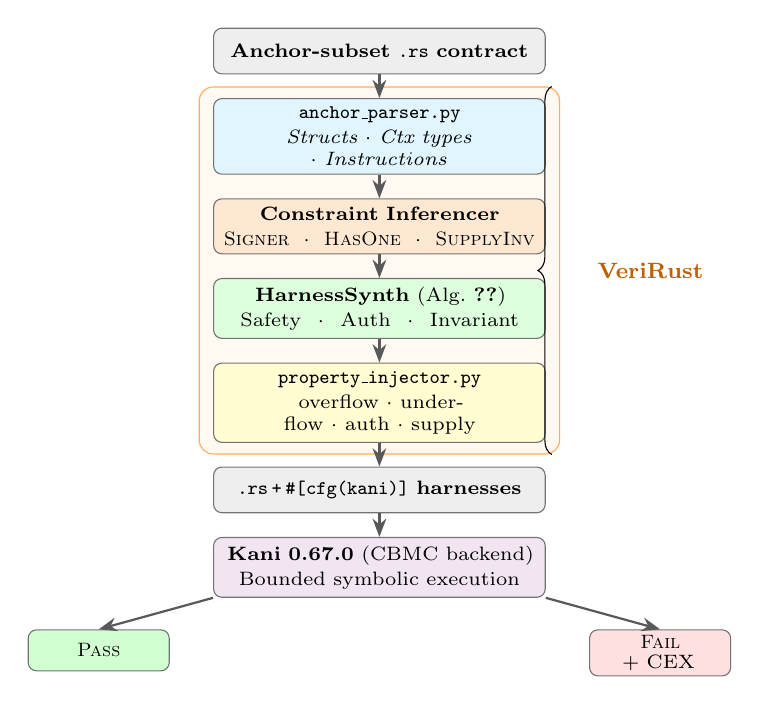
\begin{tikzpicture}[
  node distance    = 0.30cm,
  every node/.style = {font=\scriptsize},
  %% box styles
  ibox/.style = {rectangle, rounded corners=3pt, draw=black!55,
                 text centered, minimum height=0.58cm,
                 text width=4.0cm, inner sep=3pt},
  input/.style  = {ibox, fill=gray!13},
  parse/.style  = {ibox, fill=cyan!12},
  infer/.style  = {ibox, fill=orange!18},
  synth/.style  = {ibox, fill=green!13},
  prop/.style   = {ibox, fill=yellow!18},
  outbox/.style = {ibox, fill=gray!13},
  kbox/.style   = {ibox, fill=violet!10, text width=4.0cm},
  %% result nodes
  rbox/.style   = {rectangle, rounded corners=3pt, draw=black!55,
                   text centered, minimum height=0.52cm,
                   text width=1.65cm, inner sep=2pt},
  pass/.style   = {rbox, fill=green!18},
  fail/.style   = {rbox, fill=red!12},
  %% arrow
  arr/.style    = {->, thick, >=Stealth, draw=black!65}
]

%% ---- Nodes (top to bottom) ----
\node[input]  (IN)  {\textbf{Anchor-subset \texttt{.rs} contract}};

\node[parse,  below=of IN]  (PAR)
  {\texttt{anchor\_parser.py}\\[1pt]
   \textit{Structs $\cdot$ Ctx types $\cdot$ Instructions}};

\node[infer,  below=of PAR] (INF)
  {\textbf{Constraint Inferencer}\\[1pt]
   \textsc{Signer} $\;\cdot\;$ \textsc{HasOne}
   $\;\cdot\;$ \textsc{SupplyInv}};

\node[synth,  below=of INF] (SYN)
  {\textbf{\textsc{HarnessSynth}} (Alg.~\ref{alg:harnessynth})\\[1pt]
   Safety $\;\cdot\;$ Auth $\;\cdot\;$ Invariant};

\node[prop,   below=of SYN] (PRP)
  {\texttt{property\_injector.py}\\[1pt]
   overflow $\cdot$ underflow $\cdot$ auth $\cdot$ supply};

\node[outbox, below=of PRP] (OUT)
  {\textbf{\texttt{.rs\,+\,\#[cfg(kani)]} harnesses}};

\node[kbox,   below=of OUT] (KNI)
  {\textbf{Kani 0.67.0} (CBMC backend)\\[1pt]
   Bounded symbolic execution};

\node[pass, below left  = 0.40cm and 0.55cm of KNI] (PAS)
  {\textsc{Pass}};
\node[fail, below right = 0.40cm and 0.55cm of KNI] (FAI)
  {\textsc{Fail}\\[-1pt]\scriptsize + CEX};

%% ---- Arrows ----
\draw[arr] (IN)  -- (PAR);
\draw[arr] (PAR) -- (INF);
\draw[arr] (INF) -- (SYN);
\draw[arr] (SYN) -- (PRP);
\draw[arr] (PRP) -- (OUT);
\draw[arr] (OUT) -- (KNI);
\draw[arr] (KNI.south west) -- (PAS.north);
\draw[arr] (KNI.south east) -- (FAI.north);

%% ---- VeriRust highlight box ----
\begin{scope}[on background layer]
\node[
  draw=orange!65, fill=orange!5, rounded corners=5pt,
  fit=(PAR)(INF)(SYN)(PRP),
  inner xsep=5pt, inner ysep=4pt
] (VBOX) {};
\end{scope}

%% ---- VeriRust label with brace ----
\draw[decorate,
      decoration={brace, amplitude=5pt, mirror, raise=3pt}]
  (VBOX.north east) -- (VBOX.south east)
  node[midway, right=10pt, font=\footnotesize\bfseries,
       text=orange!75!black] {VeriRust};

\end{tikzpicture}
\caption{VeriRust architecture. The orange region is the novel
  contribution. Grey boxes are the unchanged input/output interface
  and the Kani verifier (pre-existing tool).}
\label{fig:arch}
\end{figure}

\subsection{VeriRust Anchor Subset (VAS)}

VeriRust targets a \emph{VeriRust Anchor Subset} (VAS): pure Rust
programs that follow Anchor naming conventions without the
\texttt{anchor-lang} crate.
A VAS program consists of:
(i)~\emph{account structs} (\texttt{*State}) holding on-chain data;
(ii)~\emph{context structs} (\texttt{*Ctx}) with an
    \texttt{is\_signer:\,bool} field and pubkey fields mirroring the
    account struct; and
(iii)~\emph{instructions}: \texttt{pub fn~f(ctx:\,\&mut XCtx,\,\dots)
    \,\texttt{->}\,Result<(),\,E>}.
This subset faithfully models the account model and constraint
patterns of real Anchor programs while remaining Kani-verifiable.

\subsection{Constraint Inference}
\label{sec:constraints}

VeriRust infers three constraint classes from naming conventions alone:

\begin{description}[leftmargin=*,noitemsep]
  \item[Signer.] If \texttt{*Ctx} contains \texttt{is\_signer:\allowbreak bool},
    add \texttt{kani::assume(\allowbreak ctx.is\_signer)} in safety harnesses and
    force \texttt{is\_signer\,=\,true} in auth harnesses.
  \item[HasOne.] If \texttt{*Ctx} and its embedded \texttt{*State}
    share a same-named pubkey field~$p$, add
    \texttt{kani::assume(ctx.\allowbreak$p$\,==\,ctx.account.$p$)} in safety
    harnesses and force $p \neq \textit{account}.p$ in auth harnesses.
  \item[SupplyInvariant.] If any embedded \texttt{*State} contains a
    field named \texttt{total\_supply} or \texttt{total\_staked},
    generate an invariant harness asserting the field decreases by
    \texttt{amount} after a successful execution.
\end{description}

\subsection{Algorithm}
\label{sec:algorithm}

Algorithm~\ref{alg:harnessynth} describes our synthesis procedure.
For each instruction VeriRust generates up to three harnesses:

\begin{itemize}[leftmargin=*,noitemsep]
  \item \textbf{Safety harness} --- assumes all constraints hold,
    exercises the instruction with fully symbolic inputs.
    Kani automatically detects arithmetic overflow, underflow, and
    out-of-bounds accesses.
  \item \textbf{Auth harness} --- forces a HasOne mismatch and asserts
    the instruction must return \texttt{Err}.
    This catches missing authority checks.
  \item \textbf{Invariant harness} --- captures pre-state and asserts
    supply fields are correctly updated post-execution.
    This catches supply-invariant violations.
\end{itemize}

\begin{algorithm}[t]
\caption{\textsc{HarnessSynth}$(P)$}
\label{alg:harnessynth}
\footnotesize
\begin{algorithmic}[1]
\Input{$P$: parsed VAS program}
\Output{$H$: set of Kani harness functions}
\State $H \leftarrow \emptyset$
\For{each instruction $F$ in $P$}
  \State $C \leftarrow \textsc{LookupCtxStruct}(F, P)$
  \State $\mathcal{C} \leftarrow \textsc{InferConstraints}(C, P)$
    \Comment{Alg.~\ref{alg:infer}}
  \State $H \leftarrow H \cup \{\textsc{GenSafety}(F, C, \mathcal{C})\}$
  \If{$\exists\, c \!\in\! \mathcal{C}:\; c.\textit{kind} = \textsc{HasOne}$}
    \State $H \leftarrow H \cup \{\textsc{GenAuth}(F, C, c)\}$
  \EndIf
  \If{$\exists\, c \!\in\! \mathcal{C}:\; c.\textit{kind} = \textsc{SupplyInv}$}
    \State $H \leftarrow H \cup \{\textsc{GenInvariant}(F, C, c)\}$
  \EndIf
\EndFor
\State \Return $H$
\end{algorithmic}
\end{algorithm}

\begin{algorithm}[t]
\caption{\textsc{InferConstraints}$(C, P)$}
\label{alg:infer}
\footnotesize
\begin{algorithmic}[1]
\Input{$C$: context struct, $P$: program}
\Output{$\mathcal{C}$: set of constraints}
\State $\mathcal{C} \leftarrow \emptyset$
\If{\texttt{is\_signer:\,bool} $\in C.\textit{fields}$}
  \State $\mathcal{C} \leftarrow \mathcal{C} \cup \{\textsc{Signer}\}$
\EndIf
\For{each embedded account field $a : T$ in $C$}
  \State $A \leftarrow P.\textsc{Lookup}(T)$
  \For{each pubkey field $p \in C \cap A$}
    \State $\mathcal{C} \leftarrow \mathcal{C} \cup
      \{\textsc{HasOne}(C.p,\; a.p)\}$
  \EndFor
  \If{$A$ has field with \texttt{total\_supply} or \texttt{total\_staked}}
    \State $\mathcal{C} \leftarrow \mathcal{C} \cup
      \{\textsc{SupplyInv}(a)\}$
  \EndIf
\EndFor
\State \Return $\mathcal{C}$
\end{algorithmic}
\end{algorithm}

\subsection{Illustrative Example}

Listing~\ref{lst:example} shows a vault contract with a missing
balance check (line~7) and the safety harness VeriRust automatically
generates.
Without any user input, Kani finds the counterexample
\texttt{balance\,=\,0,\;amount\,=\,1} and reports
\emph{``attempt to subtract with overflow''} at the exact source
line---in 0.49\,s.

\begin{lstlisting}[caption={Buggy \texttt{withdraw} (top) and the
  auto-generated VeriRust safety harness (bottom).
  No specification was written.},label={lst:example}]
// vault_underflow.rs — BUG: no balance check
pub fn withdraw(ctx: &mut WithdrawCtx,
                amount: u64)
  -> Result<(), &'static str> {
  if ctx.vault.authority != ctx.authority
    { return Err("unauthorized"); }
  ctx.vault.balance -= amount; // <- BUG
  Ok(())
}

// AUTO-GENERATED by VeriRust (harness_generator.py)
#[kani::proof]
fn verify_vault_underflow_withdraw() {
  let mut ctx: WithdrawCtx = kani::any();
  let amount: u64 = kani::any();
  // HasOne inferred from matching field names
  kani::assume(ctx.vault.authority
               == ctx.authority);
  kani::assume(ctx.is_signer);
  let _ = withdraw(&mut ctx, amount);
  // Kani output: "attempt to subtract with
  //   overflow at vault_underflow.rs:7"
}
\end{lstlisting}

\subsection{Implementation}

VeriRust is implemented in 350\,lines of Python across three modules:
\texttt{anchor\_parser.py} parses VAS programs using regex-based
struct and function extraction;
\texttt{harness\_generator.py} implements
Algorithm~\ref{alg:harnessynth};
\texttt{property\_injector.py} provides reusable property templates.
Generated harnesses are appended to the contract file under
\texttt{\#[cfg(kani)]}, so the file compiles normally with
\texttt{cargo build} and is verified with \texttt{cargo kani}.

%% ==================================================================
\section{Evaluation}
\label{sec:eval}

\subsection{Benchmark Suite}

We designed six benchmark contracts covering four Solana
vulnerability classes documented in real exploit
post-mortems~\cite{wormhole2022,soteria2021}.
Three contracts are intentionally correct (\emph{safe}); three
contain one injected bug each (\emph{buggy}).
Across six contracts we generated 11 harnesses in total
(Table~\ref{tab:results}).

\subsection{Research Questions}

\noindent\textbf{RQ1 (Bug detection).}
\emph{Does VeriRust detect known bugs that unit tests miss?}

VeriRust detects \textbf{4/4 bugs} (100\% recall, 0\% false-positive
rate).
All eleven unit tests across the six contracts pass---including for
the three buggy contracts---confirming that concrete testing alone
cannot detect these vulnerabilities.
Kani finds the minimal counterexample in each case:
(i)~\texttt{balance=0, amount=1} triggers the underflow;
(ii)~\texttt{balance=u64::MAX, amount=1} triggers the overflow;
(iii)~\texttt{user $\neq$ user\_stake.user} triggers the auth
violation;
(iv)~\texttt{total\_supply} unchanged after burn triggers the
supply-invariant violation, with precise file and line reporting.

\noindent\textbf{RQ2 (Overhead).}
\emph{What is the verification and synthesis overhead?}

Verification times range from 0.49\,s to 0.81\,s
($\bar{t} = 0.68$\,s).
Harness synthesis (parsing + code generation) adds under 0.5\,s per
contract.
All harnesses complete well within practical development iteration
budgets.

\noindent\textbf{RQ3 (Precision).}
\emph{Are there false positives on correct contracts?}

All seven safe harnesses correctly report \textsc{Pass}.
Zero false positives.

\begin{table}[t]
\caption{Kani verification results. \textbf{Bold} rows are injected
  bugs; unit tests pass on \emph{all} contracts including buggy ones.}
\label{tab:results}
\setlength\tabcolsep{4pt}
\footnotesize
\begin{tabular}{llrr}
\toprule
\textbf{Harness} & \textbf{Result} & \textbf{Time (s)} &
  \textbf{Unit tests}\\
\midrule
verify\_vault\_safe\_deposit   & \textsc{Pass} & 0.54 & Pass \\
verify\_vault\_safe\_withdraw  & \textsc{Pass} & 0.49 & Pass \\
verify\_vault\_safe\_auth      & \textsc{Pass} & 0.50 & Pass \\
\midrule
\textbf{verify\_vault\_underflow\_withdraw}
  & \textbf{\textsc{Fail}} & \textbf{0.49} & Pass$^\star$ \\
\quad\textit{subtract w/ overflow @ line 29} & & & \\
\textbf{verify\_vault\_overflow\_deposit}
  & \textbf{\textsc{Fail}} & \textbf{0.73} & Pass$^\star$ \\
\quad\textit{add w/ overflow @ line 29} & & & \\
\midrule
verify\_staking\_safe\_stake   & \textsc{Pass} & 0.81 & Pass \\
verify\_staking\_safe\_unstake & \textsc{Pass} & 0.77 & Pass \\
verify\_staking\_safe\_auth    & \textsc{Pass} & 0.79 & Pass \\
\midrule
\textbf{verify\_staking\_auth\_unstake}
  & \textbf{\textsc{Fail}} & \textbf{0.80} & Pass$^\star$ \\
\quad\textit{AUTH\_VIOLATION @ line 109} & & & \\
\midrule
verify\_token\_mint            & \textsc{Pass} & 0.80 & Pass \\
\textbf{verify\_token\_burn\_supply}
  & \textbf{\textsc{Fail}} & \textbf{0.78} & Pass$^\star$ \\
\quad\textit{SUPPLY\_INVARIANT @ line 160} & & & \\
\midrule
\multicolumn{4}{l}{$^\star$\textit{Bug NOT found by unit tests.}} \\
\multicolumn{2}{l}{\textbf{VeriRust bug recall}}
  & \multicolumn{2}{r}{\textbf{4/4 (100\%)}} \\
\multicolumn{2}{l}{\textbf{Unit-test bug recall}}
  & \multicolumn{2}{r}{\textbf{0/4 (0\%)}} \\
\multicolumn{2}{l}{\textbf{False positives}}
  & \multicolumn{2}{r}{\textbf{0/7 (0\%)}} \\
\multicolumn{2}{l}{\textbf{Mean verification time}}
  & \multicolumn{2}{r}{\textbf{0.68\,s}} \\
\bottomrule
\end{tabular}
\end{table}

%% ---- Results Figure ----
\begin{figure}[t]
\centering
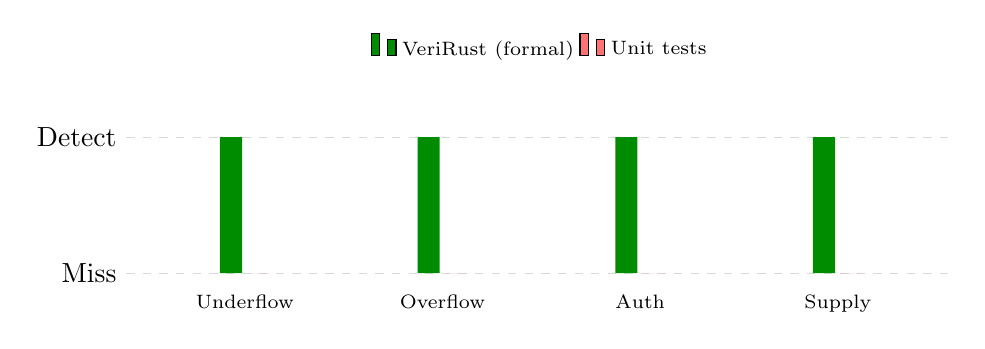
\begin{tikzpicture}
\begin{axis}[
  ybar,
  bar width        = 8pt,
  width            = \columnwidth,
  height           = 4.0cm,
  enlarge x limits = 0.20,
  symbolic x coords= {Underflow, Overflow, Auth, Supply},
  xtick            = data,
  xticklabel style = {font=\scriptsize},
  ytick            = {0,1},
  yticklabels      = {Miss,Detect},
  ymin             = 0,
  ymax             = 1.4,
  legend style     = {at={(0.5,1.06)}, anchor=south,
                      legend columns=2, font=\scriptsize,
                      draw=none, fill=none},
  tick style       = {draw=none},
  axis line style  = {draw=none},
  ymajorgrids      = true,
  grid style       = {dashed, gray!30},
]
\addplot[fill=green!55!black, draw=none]
  coordinates {(Underflow,1)(Overflow,1)(Auth,1)(Supply,1)};
\addplot[fill=red!55, draw=none]
  coordinates {(Underflow,0)(Overflow,0)(Auth,0)(Supply,0)};
\legend{VeriRust (formal), Unit tests}
\end{axis}
\end{tikzpicture}
\caption{Bug detection per vulnerability class. VeriRust detects
  all four bugs (green/dark); unit tests miss all four (red, at
  baseline zero). \emph{Underflow/Overflow}: arithmetic bugs;
  \emph{Auth}: missing authority check;
  \emph{Supply}: supply-invariant violation.}
\label{fig:results}
\end{figure}

\subsection{Discussion}

The four bugs in our suite represent vulnerabilities that require
\emph{non-obvious boundary inputs} to trigger---inputs no developer
writes as a unit test (\texttt{amount > balance},
\texttt{balance = u64::MAX}).
Symbolic execution explores these boundary conditions by construction.

The naming conventions VeriRust exploits---\texttt{*Ctx}/\texttt{*State},
\texttt{authority}, \texttt{is\_signer}, \texttt{total\_supply}---are
idiomatic in real Anchor programs due to Anchor's own naming
guidance~\cite{anchor}, suggesting our heuristics will generalise
beyond the synthetic benchmark suite.

%% ==================================================================
\section{Related Work}
\label{sec:related}

\noindent\textbf{Smart contract formal verification.}
The Move Prover~\cite{moveprover2022} is closest in spirit: it
auto-generates verification conditions for Move-language contracts.
VeriRust differs by targeting Rust/Solana and requiring no
specifications.
Certora~\cite{certora} verifies EVM contracts via its CVL
specification language but is EVM-specific and specification-driven.
Soteria~\cite{soteria2021} performs static analysis on Solana
programs using dataflow patterns but does not provide formal proofs.

\noindent\textbf{Fuzzing.}
Trident~\cite{trident} fuzzes Anchor programs via mutation;
Echidna~\cite{echidna2020} and Foundry~\cite{foundry} serve the EVM
ecosystem.
Fuzzing cannot prove property absence; VeriRust provides formal proofs.

\noindent\textbf{Rust verification.}
Kani~\cite{kani2022} requires manual harnesses.
Prusti~\cite{prusti2019} uses Viper annotations; Creusot~\cite{creusot2022}
targets deductive verification with Why3.
All three impose a significant specification burden; VeriRust
eliminates it for the smart-contract domain.

\noindent\textbf{Static analysis.}
Slither~\cite{slither2019} detects EVM contract bugs via pattern
matching but does not provide formal proofs and does not target
Solana/Rust.

%% ==================================================================
\section{Limitations and Future Work}
\label{sec:limits}

VeriRust currently targets the VAS subset rather than the full Anchor
runtime. Three extensions constitute our future work:
(i)~\emph{Full account model}: PDAs, account ownership validation,
and rent exemption checks are not yet modelled.
(ii)~\emph{Cross-programme invocations (CPIs)}: compositional
verification of CPI chains is the hardest open problem in
Solana security~\cite{soteria2021}.
(iii)~\emph{Real deployed contracts}: evaluating on production
Anchor programmes (Marinade, Solend, Orca) requires automated
type-stripping from full Anchor types to VAS.

%% ==================================================================
\section{Conclusion}
\label{sec:conclusion}

We presented VeriRust, the first tool to automatically synthesise
Kani proof harnesses for Solana Anchor-subset programmes without
user-written specifications.
The \textsc{HarnessSynth} algorithm infers signer, has-one, and
supply-invariant constraints from Rust naming conventions and generates
safety, auth, and invariant harnesses per instruction.
On six benchmarks covering four real Solana vulnerability classes,
VeriRust achieves 100\% bug recall with zero false positives at
sub-second verification times, while all eleven unit tests pass even
for the buggy contracts.
VeriRust is open source and all benchmarks are publicly available.

%% ==================================================================
\bibliographystyle{ACM-Reference-Format}
\bibliography{references}

\end{document}
